\section{Contrastive Learning and AudioCLIP}

\subsection{Contrastive Learning}
Contrastive Learning is self-supervised representation learning by training a model to differentiate between similar and dissimilar samples.\cite{ContrastiveLearning}. In few words, contrastive learning is a technique used to learn a feature space where similar samples are close together and dissimilar samples are far apart. To achieve this, a specific loss function known as \textbf{Contrastive Loss} is used:
\begin{equation}
\ell_{i,j} = -\log \frac{\exp(\text{sim}(z_i, z_j)/\tau)}{\sum_{k=1}^{2N} [k \neq i] \exp(\text{sim}(z_i, z_k)/\tau)},
\end{equation}
where $\text{sim}(z_i, z_j)$ represents the similarity between two feature vectors $z_i$ and $z_j$, $\tau$ is a temperature parameter, and $N$ is the batch size. The numerator focuses on the similarity between the positive pair $(z_i, z_j)$, while the denominator normalizes over all pairs excluding $z_i$ itself.

\begin{figure}[H]
    \centering
    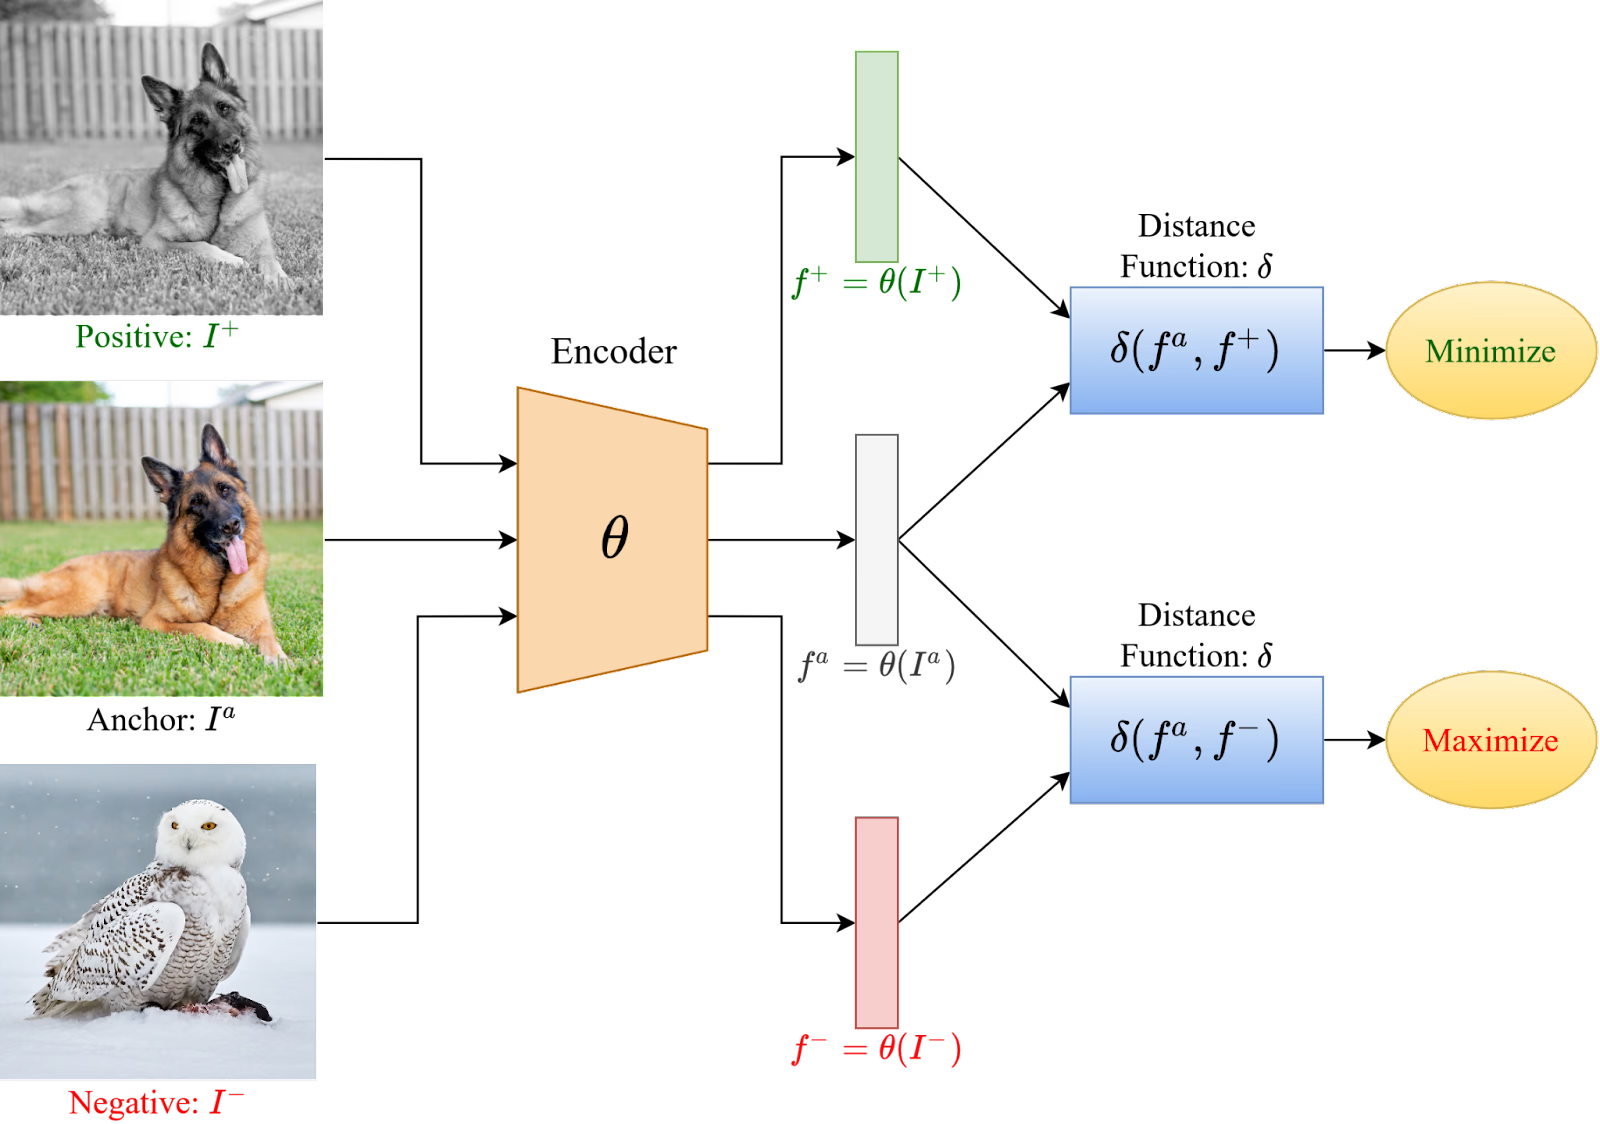
\includegraphics[width=0.8\textwidth]{img/CLearning.png}
    \caption{Conceptual representation of Contrastive Learning}
\end{figure}

\subsection{CLIP}
CLIP, which stands for Contrastive Language-Image Pre-training, is a neural network architecture developed by OpenAI\cite{CLIP} that uses Contrastive Learning to connect textual and visual information. The main idea behind CLIP is that visual and textual embeddings lives in the same feature space. Given the textual description of an image and the image itself, the embeddings returned by the model should be close together in the feature space. In few words, CLIP is trained to predict which images are most relevant to a given text prompt, and vice versa.

\begin{figure}[H]
    \centering
    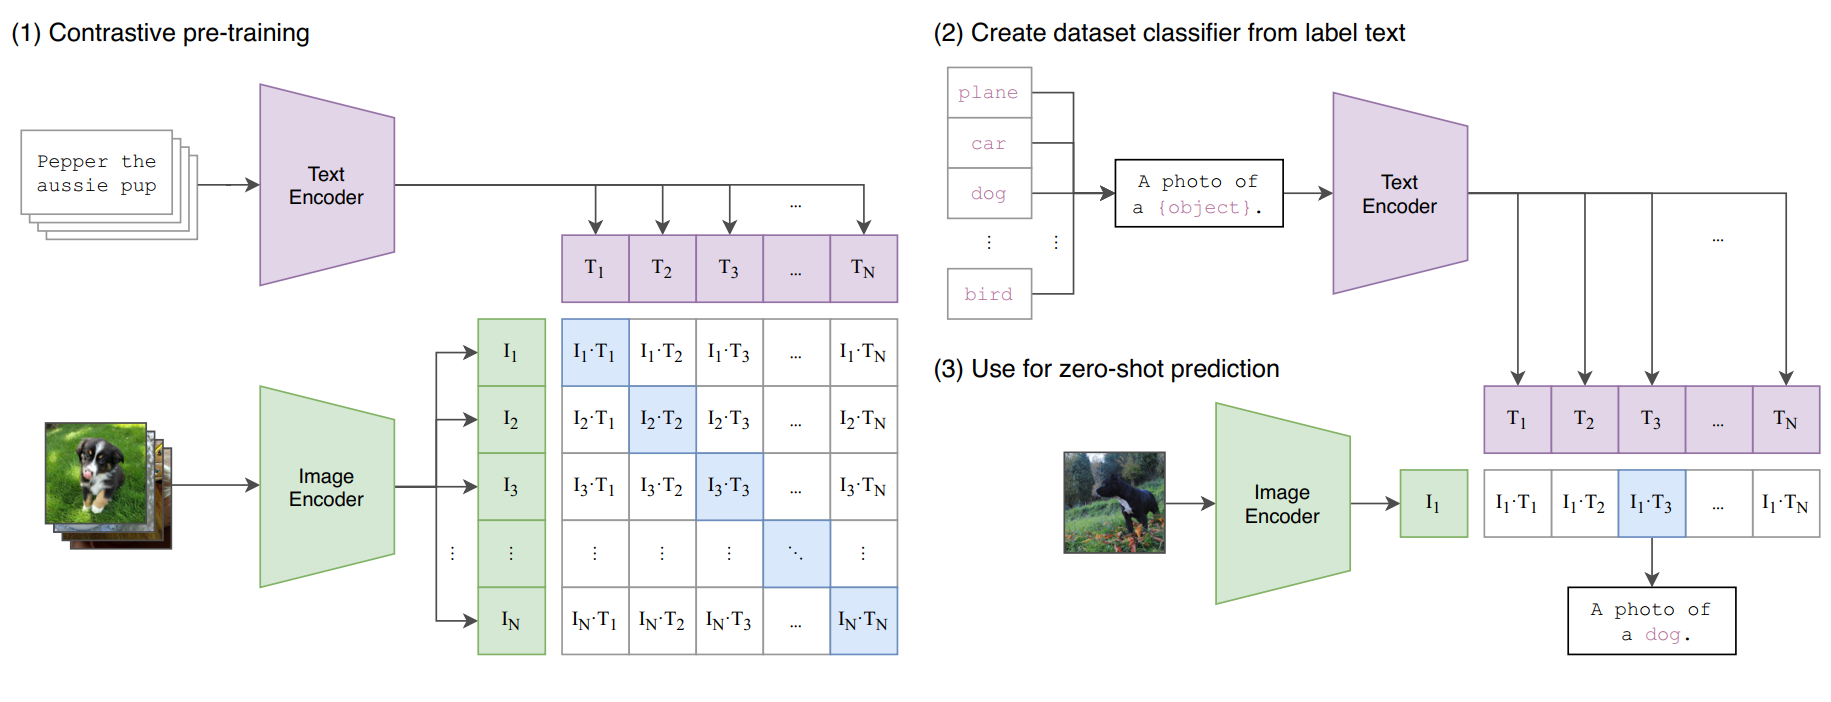
\includegraphics[width=0.8\textwidth, height=0.25\textheight]{img/CLIP.png}
    \caption{Conceptual representation of CLIP architecture}
\end{figure}

\subsection{AudioCLIP}
\label{sec:AudioClip}
AudioCLIP \cite{AudioCLIP} is an extension of the CLIP model that incorporates an additional audio modality, enabling it to understand and relate audio data alongside text and images. The architecture of AudioCLIP consists of three main components:
\begin{itemize}
    \item \textbf{A CLIP Model} to handle text and image modalities. In particual a ResNet based CLIP model is used
    \item \textbf{Audio Encoder} to handle audio modality. In particular an ESResNetXt model is used
\end{itemize}
The idea to realize AudioCLIP is very simple: in addition to the text-image contrastive loss used in CLIP, two additional loss were added: \textbf{text-audio} and \textbf{image-audio} contrastive loss. In this way the three modalities are connected in the same feature space. The training procedure of AudioCLIP consists of different main steps:
\begin{itemize}
    \item \textbf{Audio-Head Pre-Training}  
    \begin{itemize}
        \item \textbf{Standalone}: The audio head (based on ESResNeXt) is first pre-trained independently on the \textit{AudioSet} dataset.  
        \item \textbf{Cooperative}:  
        \begin{itemize}
            \item The classification layer of the pre-trained audio head is replaced with a randomly initialized layer whose output size matches CLIP’s embedding space.  
            \item The audio head is then trained jointly with the frozen text and image heads, in a \textit{multi-modal knowledge distillation} setup, making audio embeddings compatible with CLIP embeddings.
        \end{itemize}
    \end{itemize}

    \item \textbf{AudioCLIP Training}  
    \begin{itemize}
        \item After making the audio head compatible with CLIP, the entire tri-modal model (audio, text, image) is trained on \textit{AudioSet}.  
        \item All three modality-specific heads are updated together, allowing the model to adapt to the distributions of audio samples, image frames, and textual class names.  
        \item This joint training improves performance compared to training only the audio head.
    \end{itemize}
\end{itemize}


\begin{figure}[H]
    \centering
    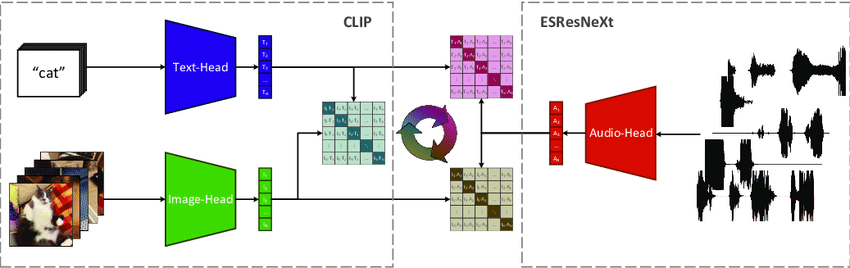
\includegraphics[width=0.8\textwidth]{img/AudioCLIP.png}
    \caption{Conceptual representation of AudioCLIP architecture}
\end{figure}